% History and Goals Slide
\section{History and Goals}
\begin{frame}{History and Goals}
  \begin{itemize}
    \item Project started in 2006 to inspire children and improve computing skills.
    \item Inspired by the BBC Micro project from 1981.
    \item Official launch: February 29, 2012, with 10,000 boards in the first run.
    \item By 2021: Over 40 million units sold, primarily manufactured in Wales.
    \item Third best-selling general-purpose computer after PC and Mac.
  \end{itemize}
\end{frame}

% Raspberry Pi Products Evolution Slide

\begin{frame}{The Raspberry Pi Products Evolution}
  \begin{itemize}
    \item Raspberry Pi 1 Model B
    \item Raspberry Pi 2/3 Model B/B+
    \item Raspberry Pi 4 Model B
    \item Raspberry Pi Zero
    \item Raspberry Pi Compute Module
    \item Raspberry Pi 5 Model B
  \end{itemize}
  \begin{center}
    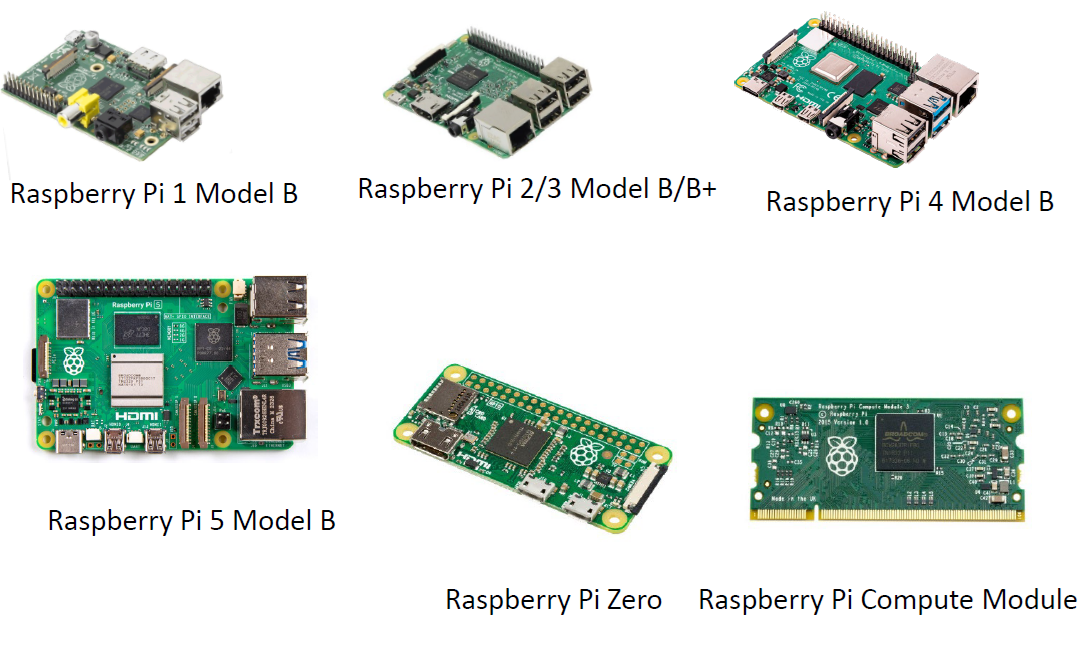
\includegraphics[width=0.8\textwidth]{trainingmaterials/rpibasics/evolution.png} 
  \end{center}
\end{frame}

% Block Diagram Slide
\begin{frame}{Block Diagram}
  \begin{center}
    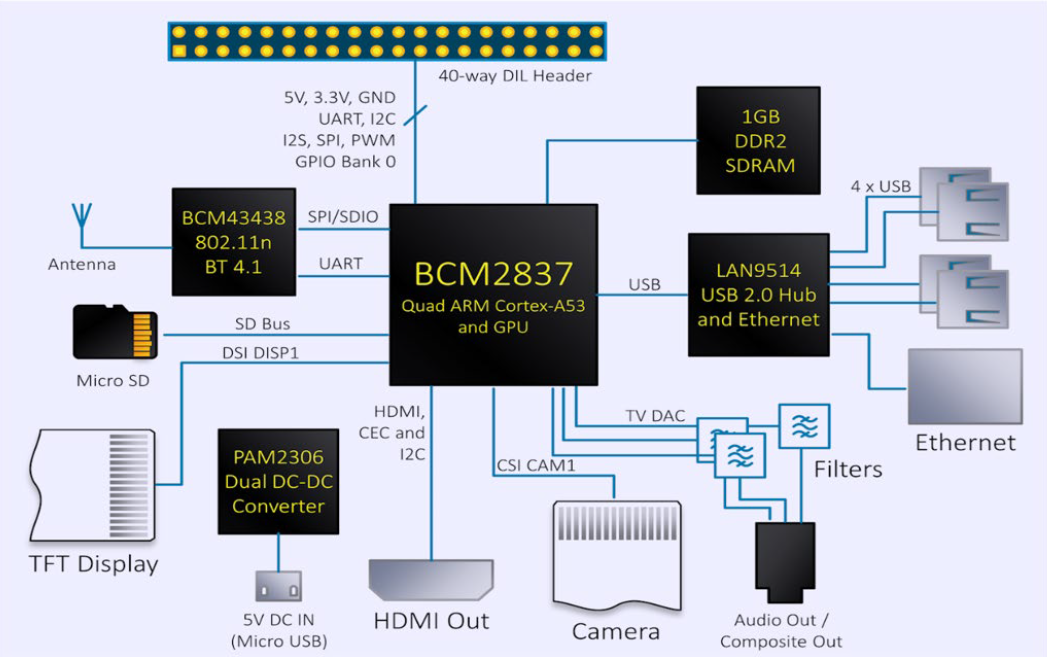
\includegraphics[width=0.8\textwidth]{trainingmaterials/rpibasics/rpiblockdiagram.png} % Replace with the actual image file
  \end{center}
\end{frame}

% Hardware Specifications Slide
\section{Hardware Specifications}
\begin{frame}{Hardware Specifications I}
  \begin{itemize}
  \item \textbf{Broadcom SoC:} Includes CPU, GPU, and DSP.
      \begin{itemize}
        \item RPI1: BCM2835, ARM 11 at 700MHz (ARMv6)
        \item RPI2: BCM2836, Quad-Core ARM Cortex A7 at 900MHz (ARMv7-A)
        \item RPI3: BCM2837, Quad-Core ARM Cortex A53 at 1.2GHz (ARMv8)
        \item RPI4: BCM2711, Quad-Core ARM Cortex A72 at 1.5GHz (ARMv8)
        \item RPI5: BCM2712, Quad-Core ARM Cortex A76 at 2.4GHz (ARMv8)
      \end{itemize}   
  \item \textbf{Memory:} The RAM is physically stacked on top of the Broadcom media processor (package-on-package technology). Ranges from 512MB (RPI1) to 8GB (RPI5).
  \item \textbf{GPU: }Provides OpenGL ES 1.1, OpenGL ES 2.0, hardware-accelerated OpenVG 1.1, Open EGL, OpenMAX and 1080p30 H.264 high-profile decode. Increase in clock frequency and 3D capabilities with the new models.
   \end{itemize}
\end{frame}

\begin{frame}{Hardware specifications II}
    \begin{itemize}
        \item LAN9512 providing: 10/100Mb Ethernet (Auto-MDIX) (RPI4 and RPI5 supports 1GbE)
        \item 2x USB 2.0 (RPI), 4 xUSB 2.0 in (RPI2/3), 2 xUSB 2.0 + 2 xUSB 3.0 (RPI4 and RPI5)
        \item Power: 5V DC (RPI 1-3 via micro-USB, RPI4/5 via USB-C)
        \item DSIinterface. 15-pin surface mounted flat flex connector, providing two data lanes, one clock lane, 3.3V and GND.
        \item HDMI connector providing type with A HDMI 1.3a out (RPI4/5 2x micro-HDMI)
    \end{itemize}
\end{frame}

\begin{frame}{Hardware specifications III}
\begin{itemize}
    \item Composite Video connector: RCA (RPI1)
     \item MIPICSI-2interface. 15-pin surface mounted flat flex connector.
     \item Audio connector: 3.5mm stereo jack (output only)
     \item SD/MMC/SDIO memory card slot (underside) (microSD since RPI2)
     \item 40-pin (2x20) 2.54 mm header expansion, providing: (26 on RPI1):
         \begin{itemize}
             \item 12 GPIOsat 3v3
            \item 2-pin UART serial console, 3v3 TTL (debug); or 2 GPIOs at 3v3
            \item I²C interface (3v3); or 2 GPIOs at 3v3
            \item SPI interface (3v3); or 5 GPIOs at 3v3
            \item 3v3, 5v and GND supply pins
            \item ARM JTAG (if pins are reconfigured in software - on Revision1.0 boards one signal would also need to be taken from S5)
            \item I²S interface (if pins are reconfigured in software, hardware hack may be required)
         \end{itemize}
\end{itemize}
\end{frame}

\begin{frame}{Hardware specifications IV}
    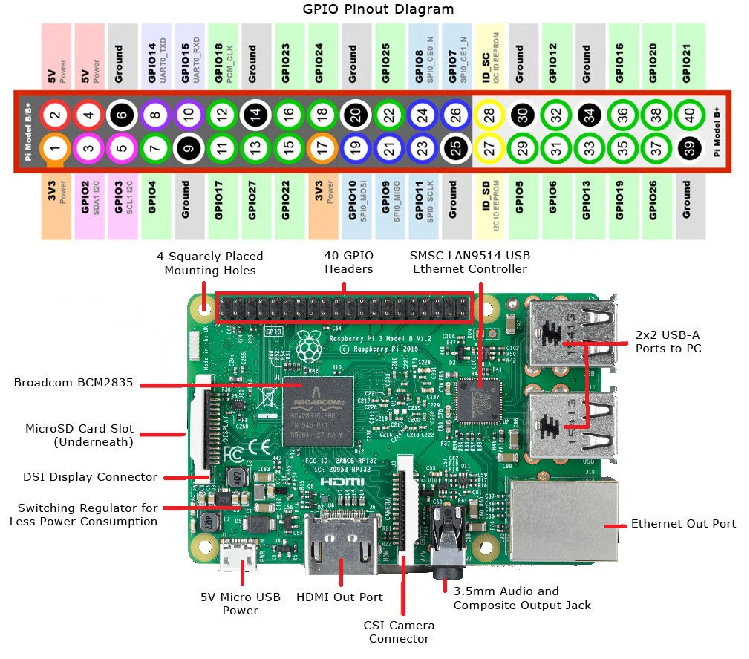
\includegraphics[scale=0.8]{trainingmaterials/rpibasics/RPIand40pin.pdf}
\end{frame}
% First Software Steps Slide
\section{First Software Steps}
\begin{frame}{First Software Steps with RPI}
  \begin{itemize}
    \item \textbf{Operating Systems:}
    \begin{itemize}
      \item Raspbian: Debian-based distribution.Linux Debian-based distribution created by Raspberry-PI organization Installation process documented in Raspberry-PI foundation website You don’t need a hard disk but an SD-Card (as faster as possible). Complete Linux with development toots and applications
      \item Ubuntu Core: Designed for IoT applications.
    \end{itemize}
    \item \textbf{Bare metal}
    \item \textbf{Software Tools:}
    \begin{itemize}
      \item GNU Compiler, linker, and debuggers for ARM processors.
      \item Programming in C and C++.
      \item Command line or Eclipse GUI.
    \end{itemize}
  \end{itemize}
\end{frame}



% Embedded Systems Slide
\section{Embedded Systems}
\begin{frame}{What are Embedded Systems?}
  \begin{columns}
      \begin{column}{0.5\textwidth}   
          \begin{itemize}
            \item Specialized computing system with specific-purpose hardware and software.
            \item Part of a larger system with real-time constraints.
            \item Examples: Router, network switch, smartphones, smartwatches, printers, gaming consoles.
          \end{itemize}
      \end{column}
  \begin{column}{0.5\textwidth} 
  \begin{center}
    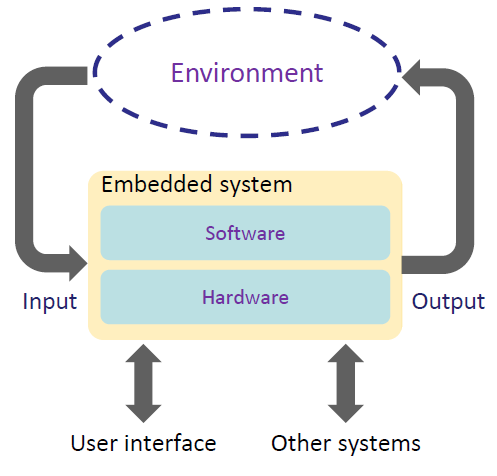
\includegraphics[width=0.8\textwidth]{trainingmaterials/rpibasics/embeddedsystem.png} 
  \end{center}
  \end{column}
 \end{columns}
\end{frame}

% Design Constraints Slide

\begin{frame}{Embedded Systems II}
\begin{columns}
      \begin{column}{0.5\textwidth} 
          \begin{itemize}
            \item Typically has a single processor core
            \item It has memory blocks, digital I/Os, analog I/Os, and communication interfaces.
            \item  Used for basic data acquisition and control purposes.
            \item  Implemented using MCUs
            \item  Integrated into mechanical or electrical systems that need real-time constraints
          \end{itemize}
        \end{column}
        \begin{column}{0.5\textwidth}
        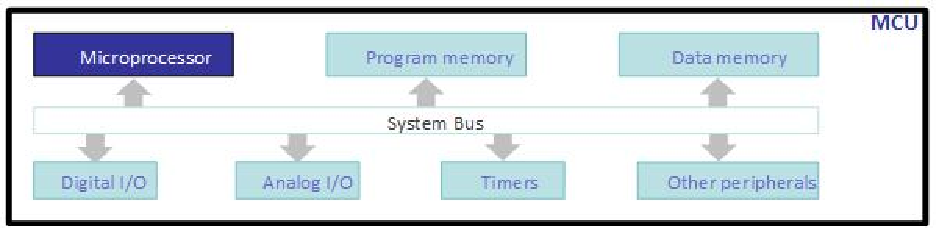
\includegraphics[width=0.8\textwidth]{trainingmaterials/rpibasics/mcu.pdf}
        \end{column}
  \end{columns}
\end{frame}

\begin{frame}{Alternatives to implement Embedded Devices}
    \centering
     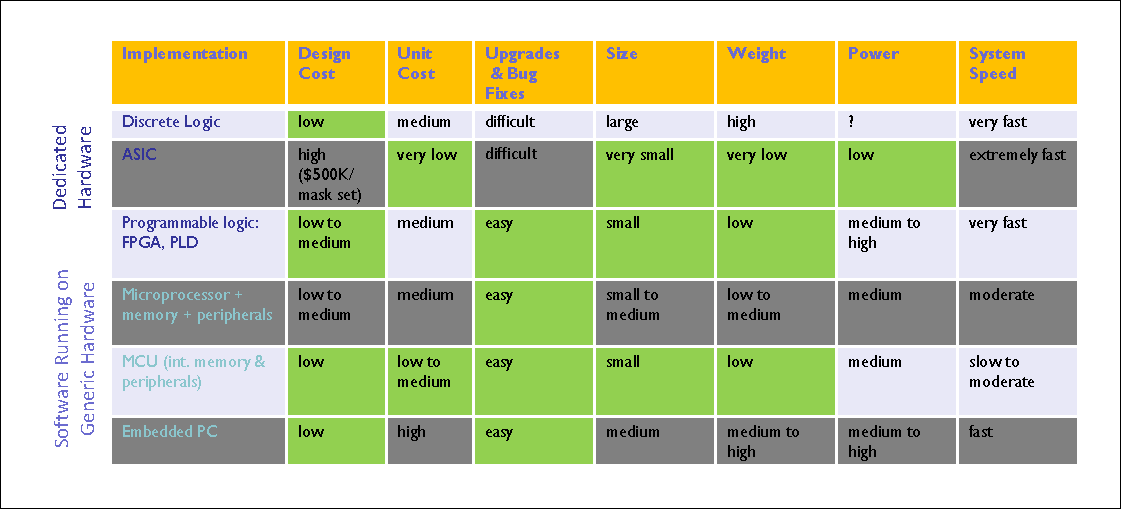
\includegraphics[width=\textwidth]{trainingmaterials/rpibasics/alternatives.pdf}
\end{frame}

\begin{frame}{Benefits of Embedded Devices}
  \begin{itemize}
    \item \textbf{Greater performance and efficiency:} More sophisticated control through software.
    \item \textbf{Lower cost:} Cheaper components. Reduced manufacturing costs. Reduced operating and maintenance costs.
    \item \textbf{More features:} Many not possible or impractical using other approaches.
    \item \textbf{Better dependability:} Adaptive systems that can compensate for failures. Better diagnostics to improve repair time.
  \end{itemize}
\end{frame}

\begin{frame}{Functions of Embedded Devices}
  \begin{itemize}
    \item \textbf{Closed-loop control system:} Monitor a process, adjust an output to maintain the desired set point of operation (temperature, speed, direction, etc.).
    \item \textbf{Sequencing:} Step through different stages based on environment and system conditions.
    \item \textbf{Signal processing:} .Remove noise, select desired signal features.
    \item \textbf{Communications and networking:} Exchange information reliably and quickly.
  \end{itemize}
\end{frame}

\begin{frame}{Constraints Specific to Embedded Devices}
  \begin{itemize}
    \item \textbf{Cost:} Competitive markets penalize products that do not deliver adequate value for money.
    \item \textbf{Size and Weight:} Mobile (aviation, automotive) and portable (e.g., handheld, wearable) systems.
    \item \textbf{Power and Energy Limits:} Battery capacity and cooling limits.
    \item \textbf{Environmental Conditions:} Operates in extreme temperatures.
  \end{itemize}
\end{frame}

\begin{frame}{The impact of constraints}
\begin{itemize}
    \item MCUs used (rather than microprocessors)
    \begin{itemize}
        \item Include peripherals to interface with other devices and respond efficiently.
        \item On-chip RAM and ROM reduce circuit board complexity and cost.
    \end{itemize}
    \item Programming language
    \begin{itemize}
        \item Programmed in C/C++ rather than in Java, resulting in smaller and faster code, making the MCU less expensive.
        \item Some performance-critical code may be in Assembly (a lower-level language).
    \end{itemize}
    \item Bare-metal \& Operating system (OS)
    \begin{itemize}
        \item Bare-metal: Typically, no OS, but instead a simple scheduler, or even just interrupts + main code (foreground/background system).
        \item If OS used, likely to be a real-time one (RTOS).
        \item Embedded Linux.
    \end{itemize}
\end{itemize}
\end{frame}


\begin{frame}{Embedded software}
\begin{itemize}
    \item Software incorporated into/aiming to control machines or devices
    \item Usually specialized for a specific hardware platform
    \item Simple, limited memory requirements
    \item Often does not require OS support $\rightarrow$ firmware
    \item Subject to timing constraints
    \item Many control functions not tied to human interaction
\end{itemize}
\end{frame}

\begin{frame}{Embedded software constraints}
\begin{itemize}
    \item Lack of abstraction: developer directly exposed to underlying hardware
    \item Responsiveness: system needs to react to external triggers in a timely manner
    \item Concurrency: multiple physical events happening at the same time must be handled
    \item Reliability: code errors can have catastrophic events in practice
    \item Efficiency: given energy \& timing budgets, optimization is required
\end{itemize}
\end{frame}

\begin{frame}{Embedded system programming and debugging}
\begin{itemize}
    \item Different options to upload/debug code on a microcontroller
    \item A range of interfaces are used to program embedded systems, including Joint Test Action Group (JTAG), Serial Wire Debug (SWD), Single Wire Interface Module (SWIM), etc.
    \item Programming consists of writing program code to nonvolatile memory (e.g., Electrically Erasable Programmable Read-Only Memory (EEPROM)) and configuring the system via fuses.
    \item Configuration bits (fuses) control key behavior of embedded hardware, e.g., clock rate, power-up timer, etc.
    \item Different debug utilities provided by software tools providers
\end{itemize}
\end{frame}

% Embedded System Design with Raspberry Pi Slide
\section{Designing with Raspberry Pi}
\begin{frame}{Embedded System Design with Raspberry Pi}
  \begin{itemize}
    \item Use an ARM multicore platform
    \item Use of embedded peripherals
    \item Sensor interface using I2C
    \item Use of Embedded Linux as Operating System
    \item Develop applications in C/C++ with the help of Linux Kernel functionalities
    \item Develop, debug, and deploy applications using:
    \begin{itemize}
        \item GNU tools
        \item Eclipse Environment
    \end{itemize}
\end{itemize}
\end{frame}

% Market Trends Slide

\section{Market Trends I}
\begin{frame}{Market Trends I}
  \begin{itemize}
    \item \centering 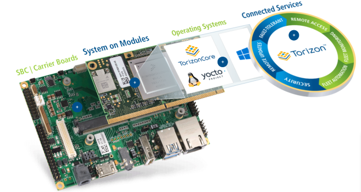
\includegraphics[scale=0.5]{trainingmaterials/rpibasics/torizon-hw.png}.
    \item 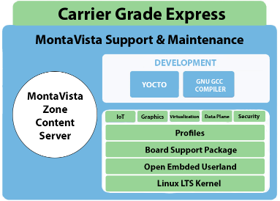
\includegraphics[scale=0.5]{trainingmaterials/rpibasics/Montavista.png}
  \end{itemize}
\end{frame}


\begin{frame}{Market Trends II}
    \begin{itemize}
        \item Industrial grade Linux
        \item Powerful features to build state-of-the-art embedded solutions
        \item Strong focus on Security with container support and services
        \item Time-saving and cost-efficient application development
        \item Drivers, connectivity stacks, real-time extensions, support for industrial hardware and graphical development environment
        \item Engineers support with experience in industrial applications
    \end{itemize}
    \begin{itemize}
        \item \centering 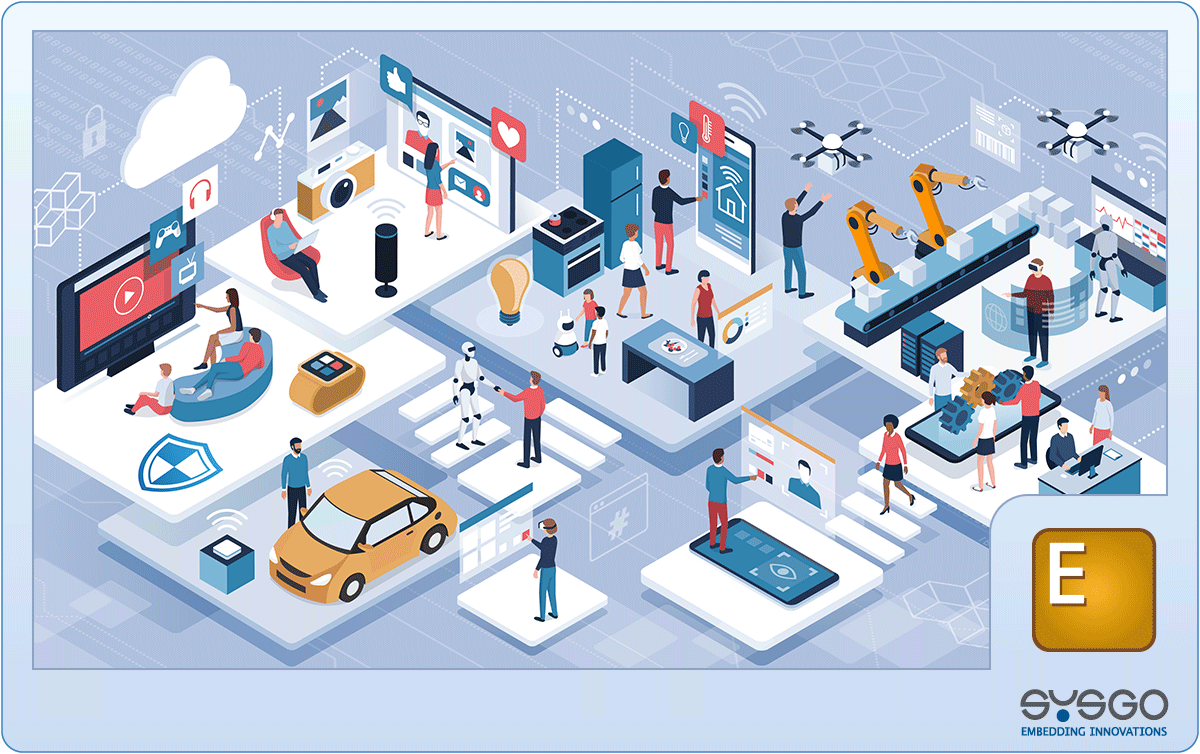
\includegraphics[scale=0.15]{trainingmaterials/rpibasics/SYSGO_graphic_elinos_embedded_linux.png}
    \end{itemize}
\end{frame}


\begin{frame}{Market Trends in Advanced Embedded Systems}
  \begin{itemize}
    \item Increasing adoption of AI engines and DSP engines.
    \item Use of adaptable hardware (e.g., Xilinx Versal, Intel Agilex).
    \item Embedded Linux plays a critical role in modern systems.
    \begin{itemize}
        \item \centering 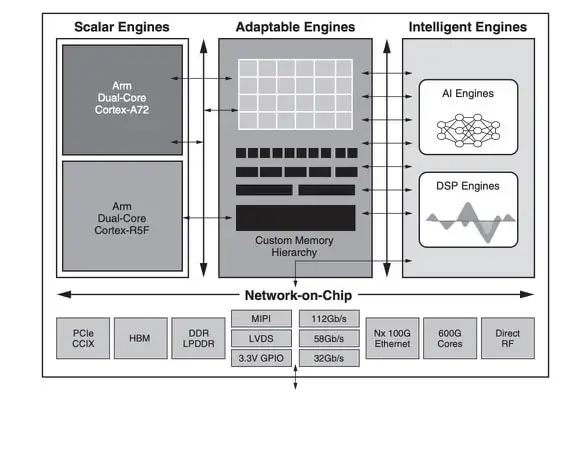
\includegraphics[scale=0.5]{trainingmaterials/rpibasics/xilinxacap.png}
    \end{itemize}
  \end{itemize}
\end{frame}

% Student Research Slide
\section{Student Research}
\begin{frame}{Student Research Topics I}
 \begin{itemize}
    \item What is the architecture of the Raspberry Pi 4 Model B+ core? Is it a 32-bit or 64-bit core?
    \item What is bare-metal programming?
    \item What software tools are required to do bare-metal programming?
    \item What are the advantages/disadvantages of using bare metal programming vs. operating system programming?
    \item What are the typical compiler and linker used in Linux OS?
    \item Review the concept of compile and link
    \item What is a library? What extensions do the library files have?
    \item What is the purpose of the Linux “make” command?
    \item What is a Makefile file?
    \item What do user space and kernel space mean in Linux?
    \item What is a GPU?
    \item What are the main advantages of using GPUs?
    \item What is the typical programming method for developing applications with GPUs?
\end{itemize}
\end{frame}


\begin{frame}{Student Research Topics II}
 \begin{itemize}
    \item Identify the steps to compile a program in GNU/Linux using gcc and g++
    \item What is the purpose of glibc library in GNU/Linux?
    \item What is the utility to debug C/C++ applications with GNU tools? 
\end{itemize}
\end{frame}